\documentclass[a4paper,11pt]{report}
\usepackage[T1]{fontenc}
\usepackage[utf8]{inputenc}
\usepackage[polish]{babel}
\usepackage{lmodern}
\usepackage{graphicx}

\title{Roznice w czasie realizacji algorytmu wypelniania stosu oraz listy w zaleznosci od implementacji}
\author{Arkadiusz Cyktor 200367}

\begin{document}
\maketitle

\begin{figure}
  1. Ponizszy wykres przedstawia zaleznosc czasu potrzebnego na wykonanie algorytmu od ilosci danych, dla stosu zaimplementowanego przy uzyciu tablicy. W tym przypradku tablica zwiekszana jest o jedno pole, za kazdym razem gdy dodawana jest nowa zmienna.
  
    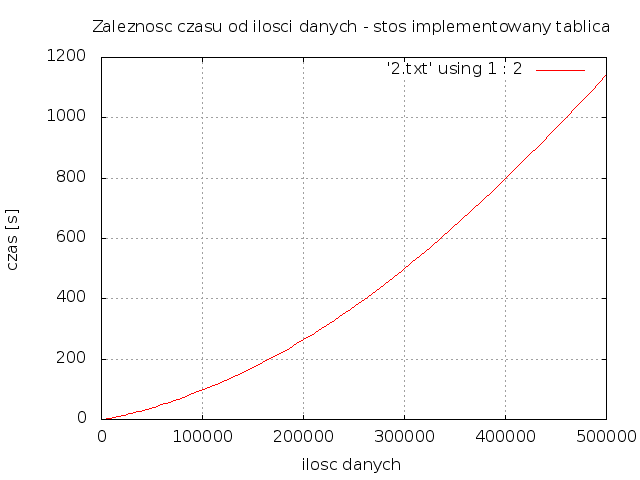
\includegraphics[scale=0.5]{./stos_tablica_o2.png}
    
    Wyniki pomiaru czasu:
  \newline  
  \begin{center}
  \begin{tabular}{|c|c|}
  \hline 
  Ilość elementów & Czas\\
  \hline
  10 & 0 \\
  \hline
  100 & 0 \\
  \hline
  1000	&	0.01 \\
  \hline
  10000	&	0.35 \\
  \hline
  100000 &	44.72 \\
  \hline
  200000 &	192.79 \\
  \hline
  300000 &	420.57 \\
  \hline
  500000 &	1142.24 \\
  \hline
\end{tabular} 
\end{center}
\end{figure}

\begin{figure}
  2. Ponizszy wykres przedstawia te sama zaleznosc dla tej samej implementacji stosu, jednak tym razem rozmiar tablicy zostaje zwiekszony dwukrotnie w momencie osiagniecia przez nia zapelnienia
  \\  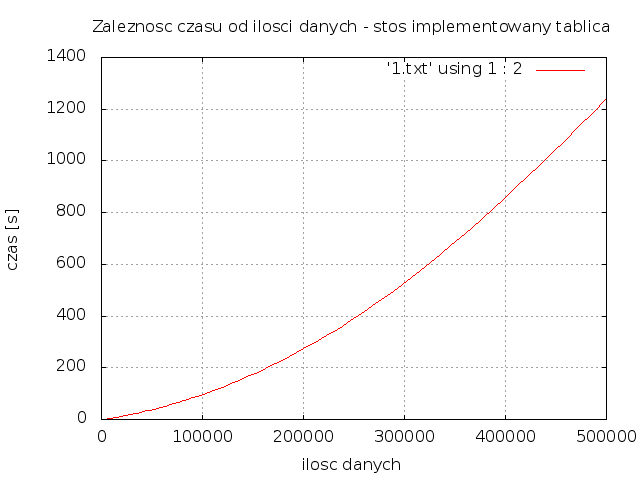
\includegraphics[scale=0.5]{./stos_tablica_o1.png}
  \\    Wyniki pomiaru czasu:
  \newline  
  \begin{center}
  \begin{tabular}{|c|c|}
  \hline 
  Ilość elementów & Czas\\
  \hline
  10 & 0 \\
  \hline
  100 & 0 \\
  \hline
  1000	&	0.01 \\
  \hline
  10000	&	0.35 \\
  \hline
  100000 &	40.4 \\
  \hline
  200000 &	183.9 \\
  \hline
  300000 &	438.08 \\
  \hline
  500000 &	1240.91 \\
  \hline
\end{tabular} 
\end{center}
\end{figure}

\begin{figure}
  3. Ponizszy wykres przedstawia zaleznosc czasu potrzebnego na wykonanie algorytmu od ilosci danych, dla stosu zaimplementowanego przy uzyciu listy.
   \\ 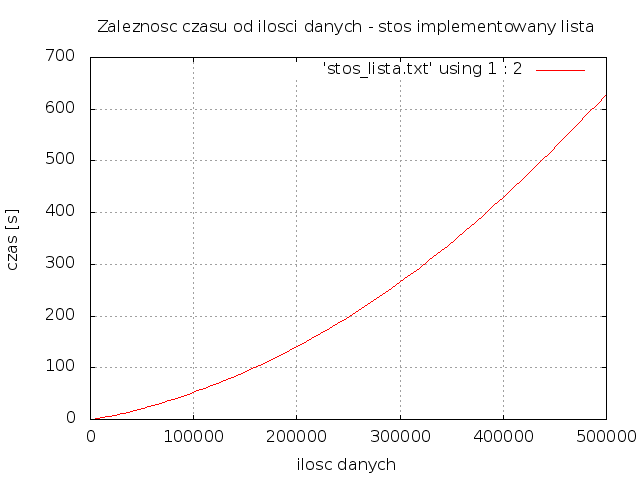
\includegraphics[scale=0.5]{./s_stos_lista.png}
    \\  Wyniki pomiaru czasu:
  \newline  
  \begin{center}
  \begin{tabular}{|c|c|}
  \hline 
  Ilość elementów & Czas\\
  \hline
  10 & 0 \\
  \hline
  100 & 0 \\
  \hline
  1000	&	0.01 \\
  \hline
  10000	&	0.21 \\
  \hline
  100000 &	21.66 \\
  \hline
  200000 &	93.85 \\
  \hline
  300000 &	220.2 \\
  \hline
  500000 &	628.68 \\
  \hline
\end{tabular} 
\end{center}
\end{figure}

\begin{figure}
  4. Ponizszy wykres przedstawia zaleznosc czasu potrzebnego na wykonanie algorytmu od ilosci danych, dla kolejki zaimplementowanej przy uzyciu tablicy.
  \\  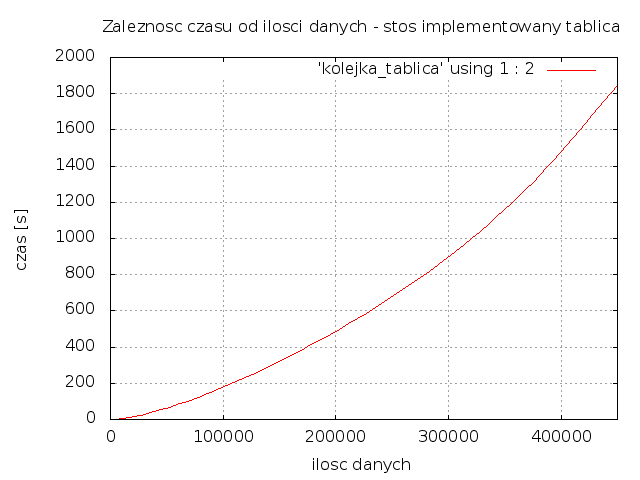
\includegraphics[scale=0.5]{./s_kolejka_tablica.png}
           \\ Wyniki pomiaru czasu:
  \newline  
  \begin{center}
  \begin{tabular}{|c|c|}
  \hline 
  Ilość elementów & Czas\\
  \hline
  10 & 0 \\
  \hline
  100 & 0 \\
  \hline
  1000	&	0.02 \\
  \hline
  10000	&	0.9 \\
  \hline
  100000 &	90.83 \\
  \hline
  200000 &	409.19 \\
  \hline
  300000 &	800.34 \\
  \hline
  450000 &	1845.09 \\
  \hline
\end{tabular} 
\end{center}
\end{figure}

\begin{figure}
  5. Ponizszy wykres przedstawia zaleznosc czasu potrzebnego na wykonanie algorytmu od ilosci danych, dla kolejki zaimplementowanej przy uzyciu listy.
   \\ 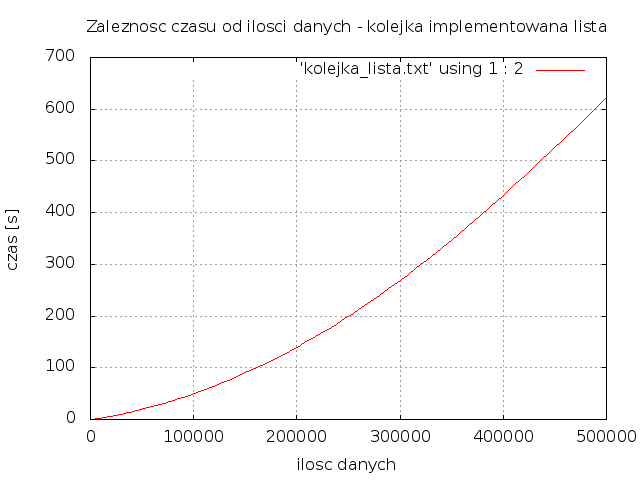
\includegraphics[scale=0.5]{./s_kolejka_lista.png}
        \\  Wyniki pomiaru czasu:
  \newline  
  \begin{center}
  \begin{tabular}{|c|c|}
  \hline 
  Ilość elementów & Czas\\
  \hline
  10 & 0 \\
  \hline
  100 & 0 \\
  \hline
  1000	&	0 \\
  \hline
  10000	&	0.21 \\
  \hline
  100000 &	21.48 \\
  \hline
  200000 &	95.07 \\
  \hline
  300000 &	226.06 \\
  \hline
  500000 &	623.15 \\
  \hline
\end{tabular}
\end{center}
\end{figure}

\begin{figure}
  6. Ponizszy wykres przedstawia zebranie wszystkich powyższych.
    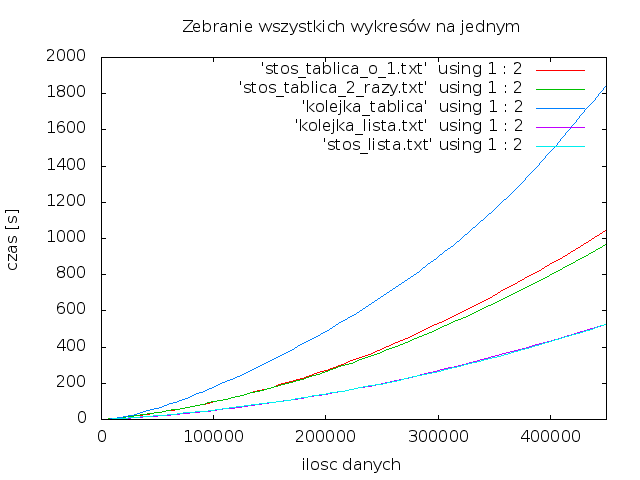
\includegraphics[scale=0.5]{./razem.png}
\end{figure}

\begin{figure}
Wnioski:
   \\- Wszystkie implementacje mają złożoność \emph{nlogn}. Na pierwszy rzut oka wykresy mogą bardziej przypominać zależność kwadratową, jednak jeśli zwróci się uwagę na tempo ich wzrostu i porówna je z zamieszczonym poniżej wykresem poglądowym, to łatwo jest zauważyć różnice (linia czerwona - \emph{n*logn}, linia zielona - \emph{n*n}.
    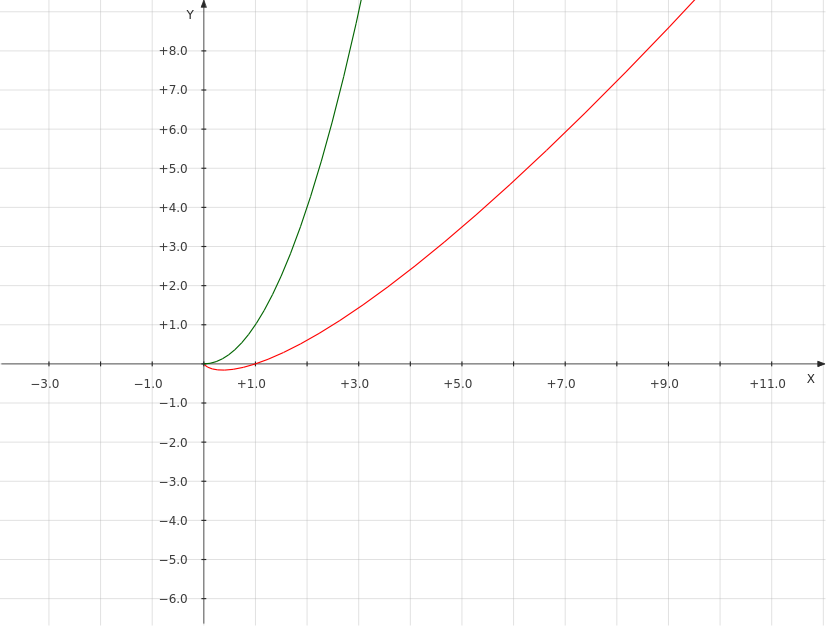
\includegraphics[scale=0.5]{./pogladowy.png}

    - Porownanie dwoch pierwszych wykresow pokazuje, ze dwukrotne zwiekszanie tablicy jest lepszym rozwiazaniem, przy pracy na duzej ilosc danych, niz rozszerzanie jej o pojedyncze pola. Mimo, ze zlozonosc obu rozwiazan rozne wykladniczo, to jednak przyrost ten jest znacznie mniejszy w przypadku drugiej metody, wymaga jednak ona znacznie wiecej pamieci.

    - Porównanie wszystkich wykresów pozwala na określenie, który z użytych algorytmów jest najwydajniejszy, a który najmniej. Jak widać największą złożonością obliczeniową charakteryszuje się kolejka implementowana przy pomocy tablicy.

    - Najbardziej wydajna okazuje się być metoda implementacji oparta o listę - zarówno stos jak i kolejka stworzone przy jej pomocy mają najmniejszą złożoność obliczeniową.

   - W środku zestawienia znalazł się stos implemenotwany tablicowo, w tym przypadku widać jednak, że powiększanie tablicy za każdym razem o jedno pole jest mniej wydajną metodą, niż dwukrtonie zwiększanie jej rozmiaru. Różnica ta nie jest widoczna przy małej ilości danych, jednak znacząco rośnie wraz ze zwiększaniem ich liczby.
\end{figure}

\end{document}
